%   % !TEX root = ../../VIII,3_Rahmen-TeX_8-1.tex
%
%
%   Band VIII, 3 N.~??A15 // AEF
%   Signatur/Tex-Datei: LH_35_09_15_020v
%   RK-Nr. 60651 (= ex 41155; ursprüngliche Zuschreibung korrigiert: RK 41154 und 41155 gehören nicht zusammen)
%   Überschrift: [De corpore tensili rumpendo ((ex: Sit linea rigida))]
%   Datierung: [Ende Januar 1683 -- 1684]
%   WZ: LEd-WZ 803006, Gegenmarke G D (= RK-WZ: 273)
%.  SZ: (keins)
%.  Bilddateien (PDF): LH_35_09_15_020v_d1, LH_35_09_15_020v_d2, LH_35_09_15_020v_d3, LH_35_09_15_020v_d4, LH_35_09_15_020v_d5, LH_35_09_15_020v_d6a, LH_35_09_15_020v_d6b (insgesamt sieben)
%
%
\selectlanguage{ngerman}%
\frenchspacing%
%
\begin{ledgroupsized}[r]{120mm}
\footnotesize
\pstart
\noindent\textbf{Überlieferung:}
\pend
\end{ledgroupsized}
\begin{ledgroupsized}[r]{114mm}
\footnotesize
\pstart \parindent -6mm
\makebox[6mm][l]{\textit{L}}%
Aufzeichnung: LH~XXXV~9,~15 Bl.~20.
Ein Blatt~4\textsuperscript{o};
Fragment eines Wasserzeichens am Blattrand:
Papier aus dem Harz.
Eine Seite auf Bl.~20~v\textsuperscript{o};
Bl.~20~r\textsuperscript{o} überliefert N.~19.
\pend
\end{ledgroupsized}
%
%
\vspace*{5mm}
\begin{ledgroup}
\footnotesize
\pstart
\noindent%
\textbf{Datierungsgründe:}\label{LH_35_09_15_020v_Datierung}
Ausschlaggebend für die Datierung der vorliegenden titellosen Aufzeichnung N.~18 ist der inhaltliche Zusammenhang mit N.~17:
Hauptziel der Untersuchung ist in beiden Texten die Bestimmung der Spannkraft, die einen elastischen Körper wie etwa eine Saite % oder ein Seil 
zum Reißen führt.
Im Hintergrund stehen bei N.~18 sowie bei N.~17 die umfangreichen Untersuchungen über die Festigkeit, die in N.~14 versammelt sind.
An einer Stelle (S.~\refpassage{LH_35_09_15_020v_aliademonstrata_yuox-1}{LH_35_09_15_020v_aliademonstrata_yuox-2}) verweist N.~18 ferner auf ein Theorem, dessen Nachweis in N.~17 erbracht wird (S.~\refpassage{LH_35_09_15_018v_aliasdemonstrata_vldj-1}{LH_35_09_15_018v_aliasdemonstrata_vldj-2}).
Demgemäß ist anzunehmen, dass N.~18 nach N.~17 verfasst wurde.
Dass beide Texte auch ungefähr zur gleichen Zeit entstanden, kann man ihren Trägern entnehmen: In beiden liegt dasselbe, von einer Papiermühle in Osterode stammende Wasserzeichen vor, das im Nachlass nach heutigem Wissensstand lediglich für die Jahre 1683 und 1684 belegt ist.\protect\index{Ortsregister}{Osterode}\protect\index{Ortsregister}{Harz}
Daher ist anzunehmen, dass auch die Aufzeichnung N.~18 \textendash\ ebenso wie N.~17 \textendash\ im Zeitraum von Ende Januar 1683 bis Ende des Jahres 1684 verfasst wurde.
\pend
\end{ledgroup}
%
%
\selectlanguage{latin}%
\frenchspacing%
%
%
\vspace*{8mm}
\pstart%
\normalsize%
\noindent%
%
\lbrack20~v\textsuperscript{o}\rbrack\ %%%% Blatt 20v
%
Sit linea\protect\index{Sachverzeichnis}{linea rigida}
\edtext{rigida}{%
\lemma{rigida}\Bfootnote{%
\textit{erg.~L}}}
\textit{AB}
in quam libere natantem in aqua\protect\index{Sachverzeichnis}{aqua}
decidendo impingat globus \textit{C}\protect\index{Sachverzeichnis}{globus impingens}
in ipsius \textit{AB} medio.
Res utique eodem redit,
ac si linea\protect\index{Sachverzeichnis}{linea rigida}
\edtext{\lbrack\textit{AB}\rbrack}{%
\lemma{\textit{C}}\Bfootnote{%
\textit{L~ändert Hrsg.}}}
in globum\protect\index{Sachverzeichnis}{globus impingens} impingeretur,
quoad ictum\protect\index{Sachverzeichnis}{ictus globi} scilicet
seu vim ruptionis,\protect\index{Sachverzeichnis}{vis ruptionis}
et quo longior erit linea \textit{AB},\protect\index{Sachverzeichnis}{linea rigida}
eo facilius tunc rumpetur in medio,
longior enim erit vectis,\protect\index{Sachverzeichnis}{vectis}
qui eam rumpere conabitur,
cum \textit{C} consideretur velut
\edtext{sustentaculum,\protect\index{Sachverzeichnis}{sustentaculum}
ut cum baculum}{%
\lemma{sustentaculum,}\Bfootnote{%
\textit{(1)}~\textbar\ cum \textit{streicht Hrsg.}~%
\textbar\ bacul
\textit{(2)}~ut cum baculum\protect\index{Sachverzeichnis}{baculus}%
~\textit{L}}}
super genu\protect\index{Sachverzeichnis}{genu} frangimus.
\pend%
\pstart%
Hinc sequitur paradoxum,\protect\index{Sachverzeichnis}{paradoxon}
nempe quo latius est scutum\protect\index{Sachverzeichnis}{scutum} aliquod,
eo facilius ictu hastae\protect\index{Sachverzeichnis}{ictus hastae}
vel globi\protect\index{Sachverzeichnis}{globus impingens} vel alio quocunque
\edtext{perforari.\protect\index{Sachverzeichnis}{perforatio}
Opus tamen}{%
\lemma{perforari.}\Bfootnote{%
\textit{(1)}~, scilicet
\textit{(2)}~. Opus tamen%
~\textit{L}}}
ista habent quodam temperamento,\protect\index{Sachverzeichnis}{temperamentum}
nam
\edtext{magna latitudo\protect\index{Sachverzeichnis}{latitudo corporis}}{%
\lemma{magna}\Bfootnote{%
\hspace{-0,5mm}\textbar~admodum \textit{gestr.}~%
\textbar\ latitudo%
~\textit{L}}}
minuit vicissim et rigiditatem,\protect\index{Sachverzeichnis}{rigiditas}
seu reddit corpus flexibilius.\protect\index{Sachverzeichnis}{corpus flexibile} \makebox[1.0\textwidth][s]{Deinde non licet pro arbitrio\protect\index{Sachverzeichnis}{arbitrium} fingere idem
\edtext{esse utrum}{%
\lemma{esse}\Bfootnote{%
\textit{(1)}~ac si
\textit{(2)}~utrum%
~\textit{L}}}
moveatur excipiens\protect\index{Sachverzeichnis}{corpus excipiens} an incidens,\protect\index{Sachverzeichnis}{corpus incidens}}
\pend
 \vspace{1.5em}%
%
  \centerline{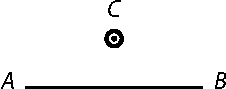
\includegraphics[width=0.26\textwidth]{gesamttex/edit_VIII,3/images/LH_35_09_15_020v_d1.pdf}}%
  \vspace{0.75em}
  \centerline{\lbrack\textit{Fig.~1}\rbrack}%
% \vspace*{1.0em}%
\newpage
\pstart\noindent
\hspace{12mm}\begin{minipage}[t]{0.5\textwidth}
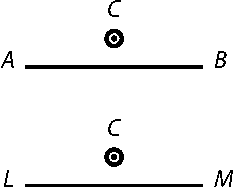
\includegraphics[width=0.58\textwidth]{gesamttex/edit_VIII,3/images/LH_35_09_15_020v_d2.pdf}
\end{minipage}
\hspace{3mm}
\begin{minipage}[t]{0.5\textwidth}
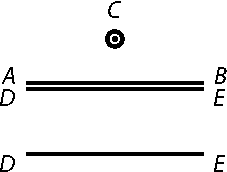
\includegraphics[width=0.56\textwidth]{gesamttex/edit_VIII,3/images/LH_35_09_15_020v_d3.pdf}
\end{minipage}\vspace{0.5em}
\\
\\
\hspace*{23mm} [\textit{Fig.~2}]\hspace*{60mm} [\textit{Fig.~3}]
\pend
\vspace{2.5em}
\pstart
\noindent\setline{1}%
ita enim potentiam\protect\index{Sachverzeichnis}{potentia} augeremus;
sed saltem ut fingamus
\edtext{amborum celeritatem esse reciprocam}{%
\lemma{amborum}\Bfootnote{%
\textit{(1)}~concursum esse aequalium vectium seu reciprocum%
\protect\index{Sachverzeichnis}{concursus vectium aequalium}
\textit{(2)}~celeritatem esse reciprocam%
~\textit{L}}}
magnitudinibus;\protect\index{Sachverzeichnis}{magnitudo corporis}
distributa hoc modo inter ipsa celeritate.\protect\index{Sachverzeichnis}{celeritas distributa}
\pend%
% \vspace*{1.5em}%
%%
%  \centerline{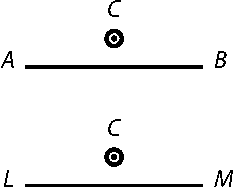
\includegraphics[width=0.26\textwidth]{gesamttex/edit_VIII,3/images/LH_35_09_15_020v_d2.pdf}}%
%  \vspace*{0.75em}
%  \centerline{\lbrack\textit{Fig.~2}\rbrack}%
%%
% \vspace*{3.0em}%
%%
%  \centerline{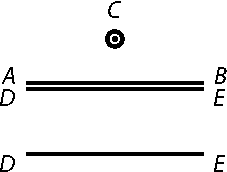
\includegraphics[width=0.26\textwidth]{gesamttex/edit_VIII,3/images/LH_35_09_15_020v_d3.pdf}}%
%%  \vspace*{0.25em}
%  \centerline{\lbrack\textit{Fig.~3}\rbrack}%
%%
% \vspace*{1.5em}%
\pstart%
Si corpus\protect\index{Sachverzeichnis}{corpus tensile}
\edtext{sit tensile,}{%
\lemma{sit}\Bfootnote{%
\textit{(1)}~flexile
\textit{(2)}~tensile,%
~\textit{L}}}
quanto longius, hoc rumpatur difficilius.\protect\index{Sachverzeichnis}{ruptura corporis}
\edtext{Ponamus globum impingere\protect\index{Sachverzeichnis}{globus impingens} in chordam}{%
\lemma{Ponamus}\Bfootnote{%
\textit{(1)}~chordam
\textit{(2)}~globum
\textit{(a)}~incidere
\textit{(b)}~impingere in chordam%
~\textit{L}}}
tensam \textit{AB},\protect\index{Sachverzeichnis}{chorda tensa}
vires globi\protect\index{Sachverzeichnis}{vis globi impingentis}
aestimandae quadrato celeritatis\protect\index{Sachverzeichnis}{quadratum celeritatis}
ductae in globum.\protect\index{Sachverzeichnis}{celeritas globi impingentis}
Debent autem vires esse ut longitudines chordarum\protect\index{Sachverzeichnis}{longitudo chordae} per
%
\edtext{\edlabel{LH_35_09_15_020v_aliademonstrata_yuox-1}%
alias demonstrata,%
\edlabel{LH_35_09_15_020v_aliademonstrata_yuox-2}}{%
\lemma{alias demonstrata}\Cfootnote{%
Siehe N.~17, S.~\refpassage{LH_35_09_15_018v_aliasdemonstrata_vldj-1}{LH_35_09_15_018v_aliasdemonstrata_vldj-2}.}}
\edtext{ergo eodem manente globo
qui suo impactu\protect\index{Sachverzeichnis}{impactus globi}
rumpere debet chordam \textit{AB}, et \textit{LM},
erunt quadrata}{%
\lemma{ergo}\Bfootnote{%
\textit{(1)}~quadrata
\textit{(2)}~eodem manente globo qui
\textit{(a)}~sua
\textit{(b)}~suo impactu \lbrack...\rbrack\ erunt quadrata%
~\textit{L}}}
celeritatum\protect\index{Sachverzeichnis}{quadratum celeritatis}
\edtext{globi perrumpentis\protect\index{Sachverzeichnis}{globus perrumpens}}{%
\lemma{globi}\Bfootnote{%
\hspace{-0,5mm}perrumpentis
\textit{erg.~L}}}
ut longitudines chordarum.\protect\index{Sachverzeichnis}{longitudo chordae}
Altitudines\protect\index{Sachverzeichnis}{altitudo lapsus} autem
ex quibus lapsus globus,\protect\index{Sachverzeichnis}{globus lapsus}
erunt ut chordae excipientes\protect\index{Sachverzeichnis}{chorda excipiens}
seu rumpendae.\protect\index{Sachverzeichnis}{chorda rumpenda}
Quaeri potest satiusne sit
\edtext{ad resistendum}{%
\lemma{ad}\Bfootnote{%
\hspace{-0,5mm}resistendum
\textit{erg.~L}}}
ex duabus chordis \textit{AB}, \textit{DE}
facere unam duplo crassiorem,\protect\index{Sachverzeichnis}{chorda duplo crassior}
ut globus\protect\index{Sachverzeichnis}{globus impingens} simul ambas rumpere debeat,
an
\edtext{vero eas separare, ita ut}{%
\lemma{vero}\Bfootnote{%
\textit{(1)}~ut
\textit{(2)}~eas separare, ita ut%
~\textit{L}}}
una perrupta\protect\index{Sachverzeichnis}{chorda perrupta}
alteram adhuc integram inveniat perrumpendam.\protect\index{Sachverzeichnis}{chorda perrumpenda}
Ita
\edtext{quidam arbitrantur,}{%
\lemma{quidam arbitrantur}\Cfootnote{%
Anspielung nicht nachgewiesen.}}
\edtext{sed rationem ejus opinionis nullam}{%
\lemma{sed}\Bfootnote{%
\textit{(1)}~cum re
\textit{(2)}~rationem ejus
\textit{(a)}~nul
\textit{(b)}~opinionis nullam%
~\textit{L}}}
reperio.
Omnis enim vis globi\protect\index{Sachverzeichnis}{vis globi impingentis}
transferri debet utique in corpus,
seu ad ejus tensionem\protect\index{Sachverzeichnis}{tensio corporis}
ruptionemve\protect\index{Sachverzeichnis}{ruptio corporis} insumi,
itaque quamdium non est insumta
\edtext{tota, operabitur}{%
\lemma{tota,}\Bfootnote{%
\textit{(1)}~restabit
\textit{(2)}~operabitur%
~\textit{L}}}
adhuc globus,\protect\index{Sachverzeichnis}{globus impingens}
nec refert itaque
\edtext{an operetur in duas chordas simul,}{%
\lemma{an}\Bfootnote{%
\textit{(1)}~simul
\textit{(2)}~operetur in duas chordas simul,%
~\textit{L}}}
quo casu cum ambae simul \makebox[1.0\textwidth][s]{sint
\edtext{tendendae,\protect\index{Sachverzeichnis}{chorda tendenda}
eo minor erit tensio\protect\index{Sachverzeichnis}{tensio chordae}
in unaquaque}{%
\lemma{tendendae,}\Bfootnote{%
\textit{(1)}~dimidi
\textit{(2)}~eo minor
\textit{(a)}~, seu
\textit{(b)}~erit tensio
\textit{(aa)}~, nempe
\textit{(bb)}~in unaquaque%
~\textit{L}}}
(\protect\vphantom)%
puto tantum fore quartam partem}
\pend
\newpage
\pstart 
\begin{minipage}[t]{0.3\textwidth}
\hspace{11mm}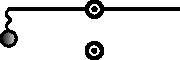
\includegraphics[width=0.68\textwidth]{gesamttex/edit_VIII,3/images/LH_35_09_15_020v_d4.pdf}
\end{minipage}
\hspace{25mm}
\begin{minipage}[t]{0.7\textwidth}
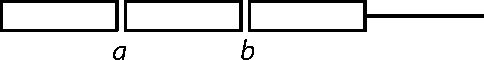
\includegraphics[width=0.55\textwidth]{gesamttex/edit_VIII,3/images/LH_35_09_15_020v_d5.pdf}
\end{minipage}
\\
\\
\hspace*{21mm} [\textit{Fig.~4, gestr.}]\hspace*{45mm} [\textit{Fig.~5, gestr.}]
\pend
\vspace{2.0em}
\pstart
\noindent tensionis%
\protect\vphantom()
\setline{1}ruptura\protect\index{Sachverzeichnis}{ruptura chordae} autem
\edtext{sequetur
cum ambae simul quaelibet ad eam tensionem\protect\index{Sachverzeichnis}{tensio chordae}}{%
\lemma{sequetur}\Bfootnote{%
\textit{(1)}~cum ambae simul ad eam ten
\textit{(2)}~cum ambae \lbrack...\rbrack\ eam tensionem%
~\textit{L}}}
perveniunt,
quae singulas rumpere potest.
Et si forte inaequalis sunt resistentiae,\protect\index{Sachverzeichnis}{resistentia ad rupturam}
unaque rumpitur ante aliam,
tunc quod reliquum virium\protect\index{Sachverzeichnis}{vis globi impingentis}
impenditur in solam nondum
\edtext{ruptam.\protect\index{Sachverzeichnis}{chorda rupta}
An ergo satis est plures}{%
\lemma{ruptam.}\Bfootnote{%
\textit{(1)}~Imo globum
\textit{(2)}~An ergo satis est
\textbar~satis est \textit{streicht Hrsg.}~%
\textbar\ plures%
~\textit{L}}}
simul
\edtext{tendere?
\edtext{Ut si globus \textit{E}
impactus in \textit{b} ipsum debeat avellere ab \textit{a},
deinde impactus in \textit{d} ipsum avellere a \textit{c},
aut vero simul incidere in \textit{b} et \textit{d}, eaque simul avellere.%
}{\lemma{Ut si \lbrack...\rbrack\ avellere}\Cfootnote{%
Die Beschreibung bezieht sich auf das Diagramm \lbrack\textit{Fig.~6b}\rbrack.}}%
}{%
\lemma{tendere?}\Bfootnote{%
\textit{(1)}~Exempli gratia globus \textit{C} simul avellere conatur \textit{a} et \textit{b}
\textit{(a)}~impetu suo, seu embolos illos educere
\textit{(b)}~simul ergo educens embolum \textit{a} et \textit{b}.
\textit{(2)}~Ponamus
\textit{(3)}~Ut si globus \textit{E}
\textit{(a)}~cadens
\textit{(b)}~impactus in \textit{b} \lbrack...\rbrack\ avellere ab \textit{a},
\textit{(aa)}~et
\textit{(bb)}~deinde
\textit{(aaa)}~incidens
\textit{(bbb)}~impactus in \textit{d} ipsum avellere a \textit{c},
\textit{(aaaa)}~quaeri
\textit{(bbbb)}~quaeri 
\textit{(cccc)}~aut vero \lbrack...\rbrack\ simul avellere.%
~\textit{L}}}
Dico si unum non potest, nec aliud posse.
Intelligo autem globum\protect\index{Sachverzeichnis}{globus impingens}
non gravitate\protect\index{Sachverzeichnis}{gravitas} agere,
ita enim progressu novas acquiret vires,\protect\index{Sachverzeichnis}{vis globi impingentis}
sed
\edtext{impetu veluti horizontali.\protect\index{Sachverzeichnis}{impetus horizontalis}
In eo tamen satius}{%
\lemma{impetu}\Bfootnote{%
\textit{(1)}~ut ho
\textit{(2)}~veluti horizontali.
\textit{(a)}~Satius
\textit{(b)}~In eo tamen satius%
~\textit{L}}}
duo conjungi in unum,
quod ita saltem neutrum rumpitur,
si non rumpenda utraque,
et ita durabilius
\edtext{est scutum.\protect\index{Sachverzeichnis}{scutum}}{%
\lemma{est}\Bfootnote{%
\textit{(1)}~opus
\textit{(2)}~scutum.%
~\textit{L}}}
Illud maxime cavendum,
ut materia scuti non sit jam nimis tensa,\protect\index{Sachverzeichnis}{materia tensa}
ita
\edtext{enim rumpetur}{%
\lemma{enim}\Bfootnote{%
\hspace{-0,5mm}\textbar~facilius \textit{gestr.}~%
\textbar\ rumpetur%
~\textit{L}}}
sufficiente vi quadam,\protect\index{Sachverzeichnis}{vis ruptionis}
quae ad minus tensam rumpendam non suffecisset.
\pend%
\vspace{1.5em} 
\pstart 
\begin{minipage}[t]{0.5\textwidth}
\hspace{18mm}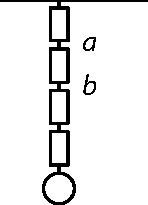
\includegraphics[width=0.22\textwidth]{gesamttex/edit_VIII,3/images/LH_35_09_15_020v_d6a.pdf}
\end{minipage}
\hspace{16mm}
\begin{minipage}[t]{0.5\textwidth}
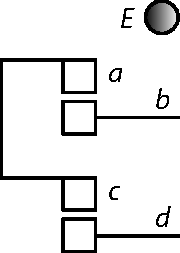
\includegraphics[width=0.35\textwidth]{gesamttex/edit_VIII,3/images/LH_35_09_15_020v_d6b.pdf}
\end{minipage}
\\
\\
\hspace*{19mm} [\textit{Fig.~6a, gestr.}]\hspace*{53mm} [\textit{Fig.~6b}]\label{LH_35_09_15_020v_d6b}
\pend
%%
%  \centerline{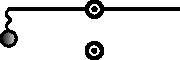
\includegraphics[width=0.21\textwidth]{gesamttex/edit_VIII,3/images/LH_35_09_15_020v_d4.pdf}}%
%  \vspace*{0.5em}
%  \centerline{\lbrack\textit{Fig.~4, gestr.}\rbrack}%
%%
% \vspace*{5.0em}%
%%
%  \centerline{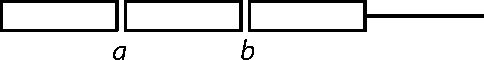
\includegraphics[width=0.40\textwidth]{gesamttex/edit_VIII,3/images/LH_35_09_15_020v_d5.pdf}}%
%  \vspace*{0.5em}
%  \centerline{\lbrack\textit{Fig.~5, gestr.}\rbrack}%
%%
% \vspace*{5.0em}%
%%
%  \centerline{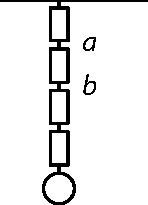
\includegraphics[width=0.13\textwidth]{gesamttex/edit_VIII,3/images/LH_35_09_15_020v_d6a.pdf}}%
%  \vspace*{0.75em}
%  \centerline{\lbrack\textit{Fig.~6a, gestr.}\rbrack}%
%%
% \vspace*{5.0em}%
%%
%  \centerline{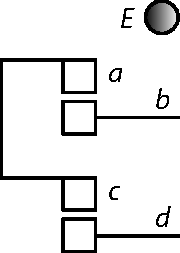
\includegraphics[width=0.19\textwidth]{gesamttex/edit_VIII,3/images/LH_35_09_15_020v_d6b.pdf}}%
%  \vspace*{0.75em}
%  \centerline{\lbrack\textit{Fig.~6b}\rbrack}\label{LH_35_09_15_020v_d6b}%
%%
%%
 \count\Bfootins=1200
\count\Afootins=1200
\count\Cfootins=1200
% ENDE DES STÜCKES auf Blatt 20v.